
\documentclass[12pt]{article}
\usepackage[margin=.9in]{geometry}
\usepackage{amsfonts}
\usepackage{amsmath,amsthm,amssymb}
\usepackage{graphicx,caption,subcaption,subfig}
\usepackage{graphics}
\usepackage[mathscr]{euscript}
\raggedright
\parindent = 0 cm
\parskip = 8pt
\numberwithin{equation}{section}

\begin{document}
\title{Reddit or Not\\ Final Report \\ Reddit }
\author{Mathew Arndt, Nicolas Bertagnolli and Micheal Matheny}
\date{}
\maketitle
\pagenumbering{arabic}
\newpage
  
\section*{Introduction}
		We had a change in direction after we realized that working with the windmill data would  be more difficult than we had imagined.  The data was so large that we could not effectively manage it in memory. This meant that our project would focus on streaming algorithms or matrix sketching.  We decided that it might be more fun to actually look at aspects of the data instead of how to work with really really big data.  This led us to switch data sets.  \newline

		This project now uses reddit data which is collected in real-time from current posts.  \newline
		
		Reddit is a very rich site where users are allowed to post just about anything.  We are interested in looking at relationships between the users of reddit and their posts.  The hope is that we might be able to uncover interesting relationships that could lead to better modeling of internet forums.  Our analysis consists of examining three different questions. The first question is, "How similar are high ranking posts?"  To asses this we use Jaccard Similarity of n-grams.  If we can uncover some degree of similarity between high ranking posts we might be able to predict if a post is going to get a lot of likes. Next we ask, "Do users post in similar categories?"  To test this idea we cluster the data based on users to see if similar users post in the same subreddits.  This will allow us to look at relationships among users.  This could lead to answer questions like is user A similar to user B.  It could also be used to create a low dimensional embedding of the users, similar to word vectors.  This might be helpful as a pretraining step in some larger learning system. Lastly we ask, "Are there words that appear frequently in specific subreddits." To test this we run Misra-Gris on the data and remove common words like "the," "and," "but," etc.  This will tell us if specific areas in reddit use common diction.  With this we might be able to identify the important words that categorize most of reddit's usage.
		
		
\section*{N-Gram Analysis (Nicolas Bertagnolli)}
	To answer the question, "how similar are high ranking posts?" we take a set of 1000 reddit posts that have over 100 up-votes from all of reddit.  The threshold was determined using domain knowledge of reddit to adequately capture a reasonably "good" post.  We validated this number by calculating the average number of up-votes on a random sample of reddit posts which turned out to be 97 up-votes.  This says that when we take posts that score above 100 we are taking posts that are above average.   The (1-4)-grams for these 1000 posts were then found and the pairwise jaccard similarity was calculated.  This number was then averaged and examined.  We found that the average Jaccard similarity between high ranking reddit posts for different n-grams was:\newline
	\begin{table}[h!]
	  \begin{tabular}{c | c c c c}
	  n-gram & 1 & 2 & 3 & 4\\
	  \hline
	  Similarity & .025 & $2.24e^{-3}$ & $1.75e^{-3}$ & $1.57e^{-3}$
	  \end{tabular}
	\end{table}
	
	These numbers are very low but they make sense because there is a great deal of variability in high ranking posts on reddit.  Take these two for example:\newline
	
	"Politics and opinions of the law aside, when a citizen has a complaint, they are encouraged to contact their representatives.  This sort of dickhead response deserves public shaming. Of course, he'll surely claim his email was hacked."\newline
	
	and \newline
	
	"If only he had another one"
	
	The first is fairly long , and the second is only a few words.  This in and of itself ensures low similarity just based on size.  Not to mention, that they both don't share a single word.  As it stands now we can say that the words alone do not make good predictors of reddit likeability.  However, there was a lot of variance in the rankings of these 1000 posts.  What happens if we restrict the posts to a range and refine our question say, "How similar are high ranking posts where the rankings differ by no more than 100 votes?"  Here we examine what happens when we take reddit posts that received between 100 and 200 up-votes.  We find that the similarities are:\newline
	
\begin{table}[h!]
	  \begin{tabular}{c | c c c c}
	  n-gram & 1 & 2 & 3 & 4\\
	  \hline
	  Similarity & .023 & $2.21e^{-3}$ & $1.69e^{-3}$ & $1.54e^{-3}$
	  \end{tabular}
	\end{table}
	This was surprising because it was slightly worse than the whole set.  This lead us to believe that a measurable amount of the similarity came from the upper upper echelon of reddit posts.This led us to examine posts that received more than 1000 votes.  We find that there is significantly more similarity among posts above 1000 up-votes.  These results are:\newline
	
	\begin{table}[h!]
	  \begin{tabular}{c | c c c c}
	  n-gram & 1 & 2 & 3 & 4\\
	  \hline
	  Similarity & .042 & .017 & .017 & .016
	  \end{tabular}
	\end{table}
	
	Now In these past experiments all possible subreddits were sampled.  This gives us an idea of similarity across all of reddit, but it seems like there is a lot of variability.  We want to see if we can better understand similarity between highly liked posts in a specific category.  For example, the posts in the funny category are probably more similar to each other than a mixture of posts from funny and say the science reddit.  We find that for the subreddits funny and science the similarities are:
	
		\begin{table}[h!]
	  \begin{tabular}{c | c c c c}
	  n-gram & 1 & 2 & 3 & 4\\
	  \hline
	  Funny & .038 & .017 & .015 & .014\\
	  Science & .494 & .397 & .394 & .394\\
	  \end{tabular}
	\end{table}
	However the Science category only had 5 results that were greater than 100
	
These results are pretty good.  They are almost on par with the above 1000 upvotes for all of reddit.  We now repeat that experiment to see if the similarity improves for extremely well liked posts the results are:

	\begin{table}[h!]
	  \begin{tabular}{c | c c c c}
	  n-gram & 1 & 2 & 3 & 4\\
	  \hline
	  Funny & .130 & .107 & .100 & .085\\
	  \end{tabular}
	\end{table}

\section*{Frequent Items Analysis (Mathew Arndt)}	
	
The question, "Are there words that appear frequently in specific subreddits?" is the problem of this section and a core mining problem.  To answer this question, the data mining seeks to find words that occur most frequent.  For each comment in the subreddit, the challenge is to collect, identify and record the most frequent words.  Since there are over one million possible words in the element space and millions of comments per year for the domain space, this problem lends itself well to a streaming algorithm.  Streaming allows the algorithm to use as little storage space as possible which is critical for such a large element and domain space.  

Focusing on words that occur most frequently, the \textbf{Heavy Hitter} algorithms were considered.  For our experiment, the \textbf{Misra-Gries} algorithm was the selected, mainly for its robustness and streaming model adaptation.  In fact, Python has a method named \textit{yield} which simply connects the parser to the Misra-Gries algorithm for recording.

On the first couple runs of the experiment, non-alphanumeric characters appeared in the words.  The original parser removed many of the non-alphanumeric characters, although several still showed up in the most frequent words(returns, brackets, backslashes, quotes etc.).  Often this created non-sense words or short phrases neither of which are the target of the mining.  As the uninvited characters showed up in the words, they were eliminated until all were weeded out.  On subsequent runs of the experiment, many lexical words appeared as the most frequent which lost the meaning of the posts.   As a remedy, a stop list was created with a list of words to be ignored.  This list was modified twice more.  First, the original list had to be duplicated because \textit{title case} continued to appear in the words.  And, second, the conjunctions were added to the stop list.  For our experiments, numbers and proper names were not added to the stop list for they often provide meaning, especially for certain subreddits.  Nevertheless, some experiments may consider removing these elements depending on the purpose of the mining.

Part of the experimental design was the selection of subreddits from which to mine.  With thousands of subreddits to select from, this is no trivial task.  Some of the more popular subreddits are \textit{funny, pics, videos, etc.}  The selection approach here was simple:  select subreddits that were popular yet had a concept that could be identified by its frequent words (topical bias hopefully excluded).   With that criteria in mind, experiments were run on the following subreddits: 

\begin{itemize} \itemsep1pt \parskip0pt \parsep0pt

  \item worldnews
  \item science
  \item funny
  \item movies
  \item aww
  \item gaming
  \item technology
  
\end{itemize}

Not all subreddits are as popular or as dense as the others.  Better results occur when the mining is allowed to traverse the comments in the subreddit to completion or near completion.  The algorithm was allowed to run until timeout.  

\begin{table}[h!]
\begin{tabular}{ll}
\textbf{subreddit} & \textbf{comments} \\
 \hline
funny              & 64,000           \\
worldnews          & 63,000           \\
gaming             & 51,000           \\
movies             & 39,000           \\
technology         & 22,000           \\
aww                & 16,000           \\
science            & 11,000          
\end{tabular}
\end{table}



For displaying the results, both tabular and histogram forms were considered.  In the end, a pictoral representation of the results was deemed best.  A \textit{wordle}, also known as a \textit{word cloud}, is such a representation where  greater prominence is given to words that appear more frequently.  Here is an example of one of the experiments run: 

The first \textbf{worldle} comes from the Misra-Gries output on the \textit{movies} subreddit:

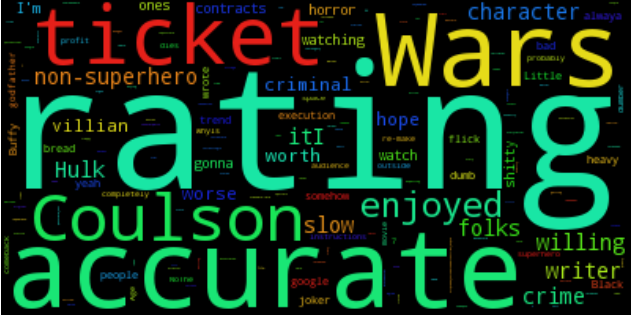
\includegraphics[scale=.5]{movies.png}

The second \textbf{worldle} comes from the Misra-Gries output on the \textit{movies} subreddit:

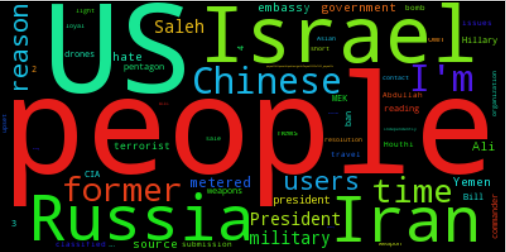
\includegraphics[scale=.5]{worldnews.png}

The \textbf{Misra-Gries} algorithm not only takes as input the stream of words but also the number of available counters, \textit{k}.  The number of counters has direct consequences on the accuracy of the Misra-Gries algorithm and also the number of words recorded and displayed.  The following shows the inverse relationship of the number of available counters and the error.    

$k=\frac { 1 }{ \varepsilon  } $  

or, in terms of error 

$\varepsilon =\frac { 1 }{ k  } $ 

For our experiments, a tradeoff exists between the accuracy in the algorithm and the amount of word clutter in the output.  In the end, the number of counters selected was two hundered, producing clean output and just a 0.5 percent error.

A basic rundown of the results of the experiments are as follows:

<table coming here>


Overall, the algorithm performed efficiently on the stream.  The main bottleneck was connecting to Reddit and the limitation on accessing the comments.  The stopwords did have an affect on which words were selected.  Short phrases might be more meaningful than single words because some context is lost in the concepts.  Also, the results were not as general as might be expected.  Proper names and places often showed up in the higher word frequency.  The \textit{k} = 200 worked well and produced clear wordles.  The main topic of the subreddit could possibly be determined by the most frequent words which is a good indicator of the effectiveness of the algorithm.   




\end{document}